\hspace{24pt}

This chapter explains the details of the experiments. It includes the use of datasets (Section~\ref{sec:dataset}), the experimental environment (Section~\ref{sec:environment}), the parameters of the NMT model (Section~\ref{sec:parameter}), and the metrics (BLEU score) of the NMT model (Section~\ref{sec:metric}). Lastly, the BLEU scores of the translation system based on different tokenizations and word embeddings are shown in Section~\ref{sec:result}.

\section{Dataset} \label{sec:dataset}

Our datasets are acquired from the Asian Scientific Paper Excerpt Corpus (ASPEC) \cite{nakazawa-etal-2016-aspec} provided by the Japan Science and Technology Agency (JST) and the National Institute of Information and Communications Technology (NICT). ASPEC consists of a Japanese-English corpus (ASPEC-JE) with 3 million parallel sentences and a Japanese-Chinese corpus (ASPEC-JC) with 680,000 pairs.

We have selected ASPEC-JC as the dataset for our zh-ja NMT system, and the structure of the dataset is shown in Table~\ref{tab:aspec-jc}. ASPEC-JC is constructed by manually translating the excerpts of Japanese scientific papers into Chinese. Papers used for translation are derived from the Japan Science and Technology Agency (JST) or the Japan Science and Technology Information Aggregator, Electronic (​J-STAGE).

\vspace{0.4cm}
\begin{table}[h]
    \centering
    \begin{tabularx}{\textwidth}{bbb}\toprule
        Data Type & File Name & Number of sentences \\\midrule
        Train & train.txt & 672,315 \\
        Validation & dev.txt & 2,090 \\
        Validation-Test & devtest.txt & 2,148 \\
        Test & test.txt & 2,107 \\
        \bottomrule
    \end{tabularx}
    \caption{ASPEC-JC dataset}
    \label{tab:aspec-jc}
\end{table}

\section{Environment} \label{sec:environment}

We use \texttt{PyTorch} \footnote{https://pytorch.org/} and \texttt{PyTorch-Lightning} \footnote{https://www.pytorchlightning.ai/} \cite{falcon2019pytorch}  as the main framework for constructing the entire NMT model (Section~\ref{sec:lightning}), as well as Weights \& Biases (wandb) \footnote{https://wandb.ai/site} \cite{wandb} for logging models, metrics, and dataflow (Section~\ref{sec:wandb}).

\subsection{PyTorch and PyTorch Lightning} \label{sec:lightning}

\texttt{PyTorch} has been widely used in academic research and production. We use \texttt{PyTorch} as a framework for processing data and designing the components (i.e., encoder, attention, decoder) of attention-based Bi-GRU Model and Transformer.

\texttt{PyTorch-Lightning} offers many advantages as a wrapper for \texttt{PyTorch}: Dataflow can be integrated more efficiently in \pythoninline{LightningDataModule}; the main source code, including the components designed by \texttt{PyTorch}, can be integrated into \pythoninline{LightningModule}; using \pythoninline{Trainer} can directly utilize the \pythoninline{LightningDataModule} and \pythoninline{LightningModule}, and help us use the correct engineering code such as gradient update, data transfer between CPU and GPU. In addition, \texttt{PyTorch-Lightning} provides a lot of plugins to simplify research, such as multi-GPU or TPU training, checkpointing and logging of models, implementing 16-bit precision, early stopping, finding learning rate and batch size, etc.

\subsection{Weights and Biases (wandb)} \label{sec:wandb}

\texttt{Wandb}, similar to \texttt{Tensorboard} \footnote{https://www.tensorflow.org/tensorboard}, is a powerful tool for logging model training and is used by OpenAI \footnote{https://wandb.ai/site/articles/why-experiment-tracking-is-crucial-to-openai}, the company designed GPT-3. \texttt{Wandb} can visualize all training metrics and system performance, record hyperparameters used in the experiments for easy replicating, integrate dataset in the cloud to facilitate the advantages of cross-platform. In the experiments, we use the \pythoninline{WandbLogger} provided by \texttt{PyTorch-Lightning} to integrate \texttt{wandb} and record the experimental results of all models, which will be presented in Section~\ref{sec:result}.

\section{Parameter} \label{sec:parameter}

We implement eight ($2\!\times\!4$) experiments for attention-based Bi-GRU Model and Transformer experiments.
The experiments use two different methods for tokenization. one using SentencePiece for both Chinese and Japanese, and the other using Jieba and Janome for Chinese and Japanese respectively. Every experiment validates four scenarios, which are the model without any pre-trained embedding (i.e., the baseline), the model using only semantic embedding, the model using only phonetic embedding, and the model using joint semantic-phonetic embedding.

Some parameters are identical in all experiments. The dataset has 50,000 sentence pairs which filtered (described in Section~\ref{sec:corpus_filtering}) and sampled by Python \pythoninline{random} module. The dictionary size for tokenizer and embedding is fixed to 32,000 and the dimension of embedding is fixed to 300. The other hyperparameters are listed in Table~\ref{tab:hyperparameters}.

\vspace{0.4cm}
\begin{table}[h]
    \centering
    \begin{tabularx}{\textwidth}{bbb}\toprule
        Hyperparameters & Attention-based Bi-GRU & Transformer \\\midrule
        dropout & 0.1 & 0.1 \\
        hidden\_dim (pf\_dim) & 512 & 512 \\
        learning rate & 7e-4 & 5e-4 \\
        precision & 16 & 32 \\
        attention heads & - & 6 \\
        layers & 1 & 3 \\ 
        \bottomrule
    \end{tabularx}
    \caption{The hyperparameters}
    \label{tab:hyperparameters}
\end{table}

Catastrophic forgetting \cite{kirkpatrick2017overcoming} may occur during training with pre-trained embedding. In other words, the gradients in the first few batches will drastically change the embeddings and lose the initial meaning from vectors completely. We overcome the problem by freezing the weights of embeddings in the first $n$ epochs, and fine-tuning the embeddings in the subsequent epochs. Therefore, $n$ is also a hyperparameter of attention-based Bi-GRU Model and Transformer. We apply $n=3$ to RNN and $n=1$ to Transformer to achieve the best results.

\section{Metric} \label{sec:metric}

We evaluated our zh-ja NMT system using the BLEU (Bilingual Evaluation Understudy) score \cite{papineni2002bleu}. The BLEU score is a number from 0 to 100 that measures the similarity between translated sentences from model and high-quality reference translations. A score of 0 means there is no overlap between machine translation and reference translation, and a score of 100 means a complete overlap between the two. A common interpretation of the BLEU score can be referred to Table~\ref{tab:bleu_score_interpretation}.

\vspace{0.4cm}
\begin{table}[h]
    \centering
    \begin{tabularx}{\textwidth}{p{3cm}b}\toprule
        BLEU Score & Interpretation \\\midrule
        $< 10$ & Almost useless \\
        $10 - 19$ & Hard to get the gist \\
        $20 - 29$ & The gist is clear, but has significant grammatical errors \\
        $30 - 40$ & Understandable to good translations \\
        $40 - 50$ & High quality translations \\
        $50 - 60$ & Very high quality, adequate, and fluent translations \\
        $> 60$ & Quality often better than human \\
    \end{tabularx}
    \caption[Interpretation of the BLEU score]{Interpretation of the BLEU score\protect\footnotemark}
    \label{tab:bleu_score_interpretation}
\end{table}

\footnotetext{Source: https://www.cs.cmu.edu/~alavie/Presentations/MT-Evaluation-MT-Summit-Tutorial-19Sep11.pdf}

Mathematically, the BLEU score is defined as eq. \ref{eq:eq16} and eq. \ref{eq:eq17}. The formula consists of two parts: the brevity penalty and the n-gram overlap. The brevity penalty penalizes the sentences that were translated too short, which were easier to score higher because of the lower denominator (in eq. \ref{eq:eq17}) calculated by n-gram. The n-gram overlap counts the number of overlaps between the translated sentences and the corresponding unigrams, bigrams, trigrams, and four-grams in the reference translation ($\text{Count}_\text{clip}$). Unigrams account for the adequacy and longer n-grams account for the fluency of the translation.

\begin{equation}
    \mathrm{BLEU}=\underbrace{\min \left(1, \exp \left(1-\frac{\text { reference-length }}{\text { output-length }}\right)\right)}_{\text {brevity penalty }} \underbrace{\left(\prod_{i=1}^{4} \text { precision }_{i}\right)^{1 / 4}}_{\text {n-gram overlap }} \label{eq:eq16}
\end{equation}

\begin{equation}
    \text { precision }_{n} = \frac{\sum_{ \text {n-gram} \in C} \text {Count}_{\text {clip}}(\text {n-gram})}{\sum_{\text{n-gram}^{\prime} \in C^{\prime}} \operatorname{Count}\left(\text{n-gram}^{\prime}\right)} \label{eq:eq17}
\end{equation}

Here are several considerations for evaluating translation models using the BLEU score. First, BLEU is a corpus-based metric that requires evaluating multiple sentences (corpus) at once; the score for individual sentences will lose some meaning; in other words, statistics are accumulated across the sentences when computing the score. Second, BLEU cannot distinguish the errors between the function words and the content words; dropped function words such as ``a'', ``the'', and ``of'' carry the same penalties as important content words that are mistranslated or lost. Third, BLEU is not good at capturing the meaning and grammaticality of sentences; namely, the impact of single words such as ``not'' that can dramatically change the semantics, and long-range dependencies of distances greater than the length of the n-gram will be underestimated.


\section{Result} \label{sec:result}

All NMT models are trained based with a dictionary size of 32,000,
300-dimensional embedding, and sampled dataset that has 50,000 sentence pairs. We first examine the losses and BLEU scores produced by different tokenization methods and embeddings on the two models. Although there is no exact correspondence between the loss and the BLEU score, the loss is still a useful metric for evaluating the performance of models such as detecting overfitting. Finally, we look into the result using the best model and the complete, filtered dataset (462,582 sentence pairs) and compare it with other studies.

\subsection{Attention-based Bi-GRU Model}

Figure~\ref{fig:seq2seq_loss} shows the losses of using the two tokenization methods on the attention-based Bi-GRU model respectively. In both Figure~\ref{fig:seq2seq_loss_sp} and \ref{fig:seq2seq_loss_jj}, it is observed that using any pre-trained embedding can effectively resist the overfitting that occurs in the baseline. Moreover, the loss of all three embeddings in Figure~\ref{fig:seq2seq_loss_sp} is similar, but the loss of joint embedding in Figure~\ref{fig:seq2seq_loss_jj} is the lowest.

\begin{figure}[t]
    \centering
    \begin{subfigure}[b]{0.495\textwidth}
        \centering
        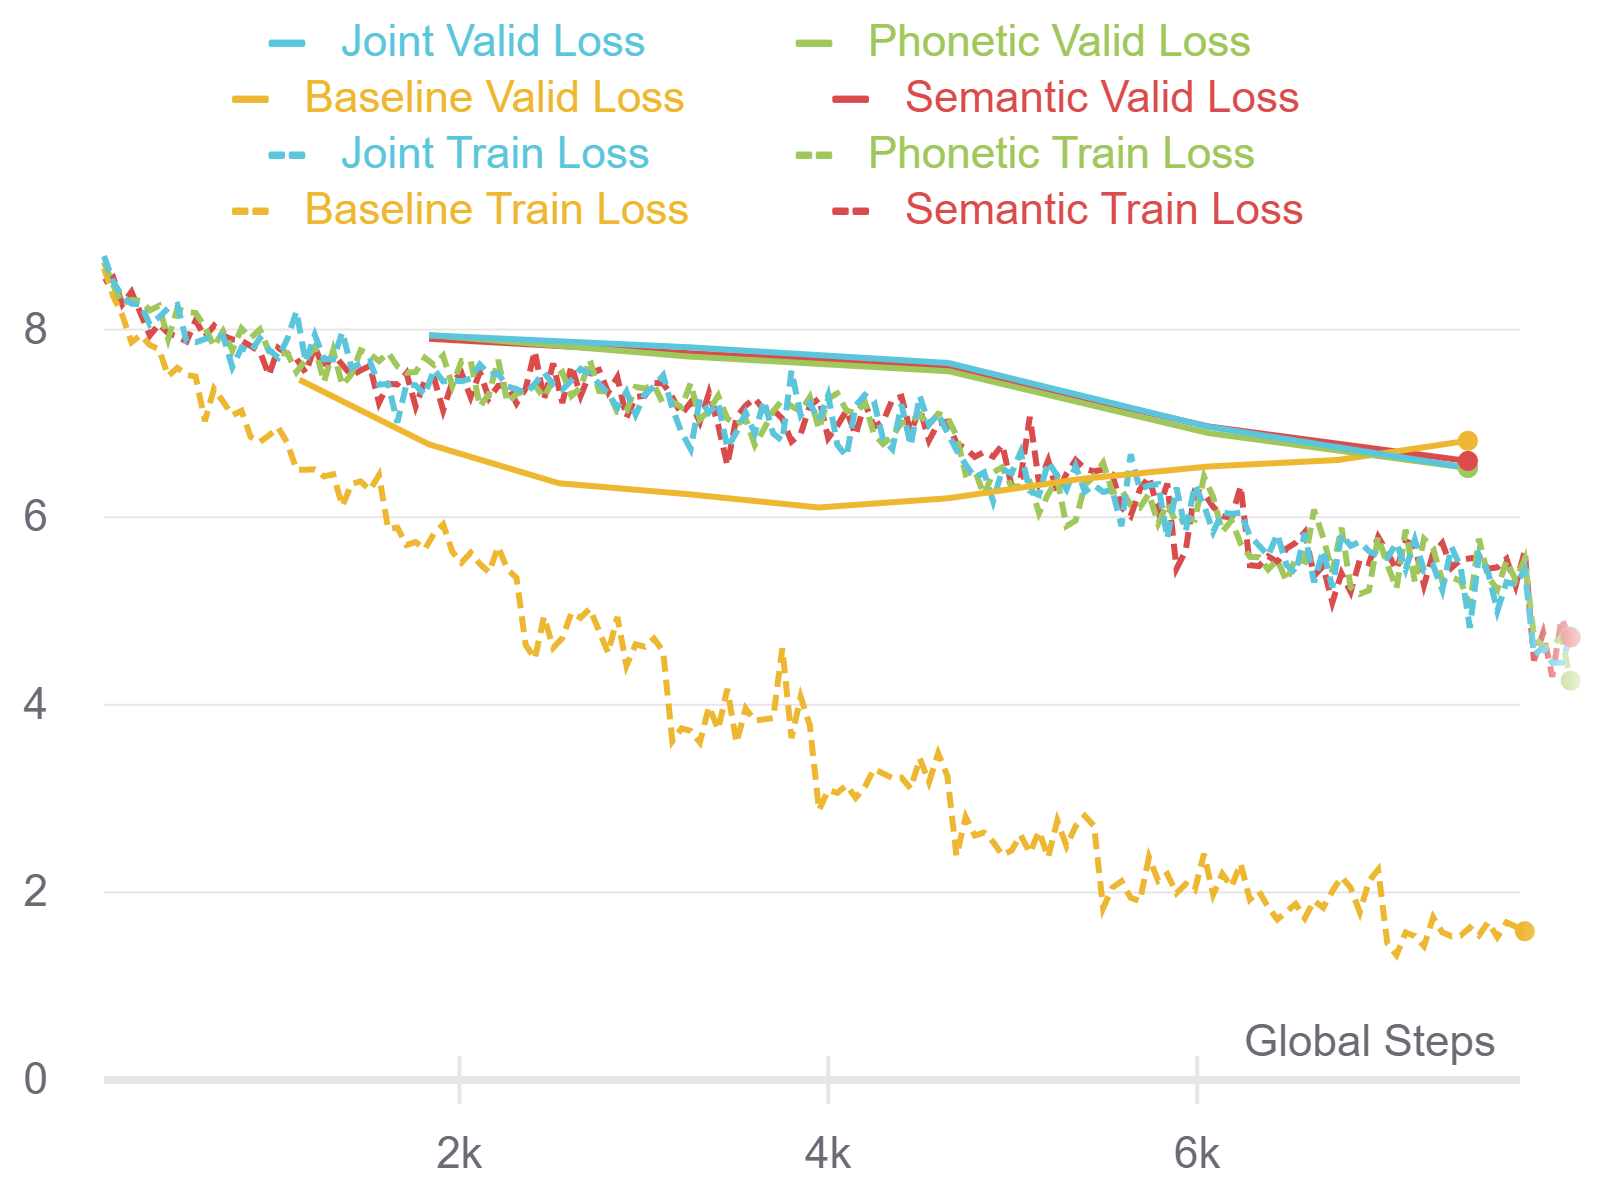
\includegraphics[width=\textwidth]{../images/rnn_sp.png}
        \caption{Results using SentencePiece}
        \label{fig:seq2seq_loss_sp}
    \end{subfigure}
    \hfill
    \begin{subfigure}[b]{0.495\textwidth}
        \centering
        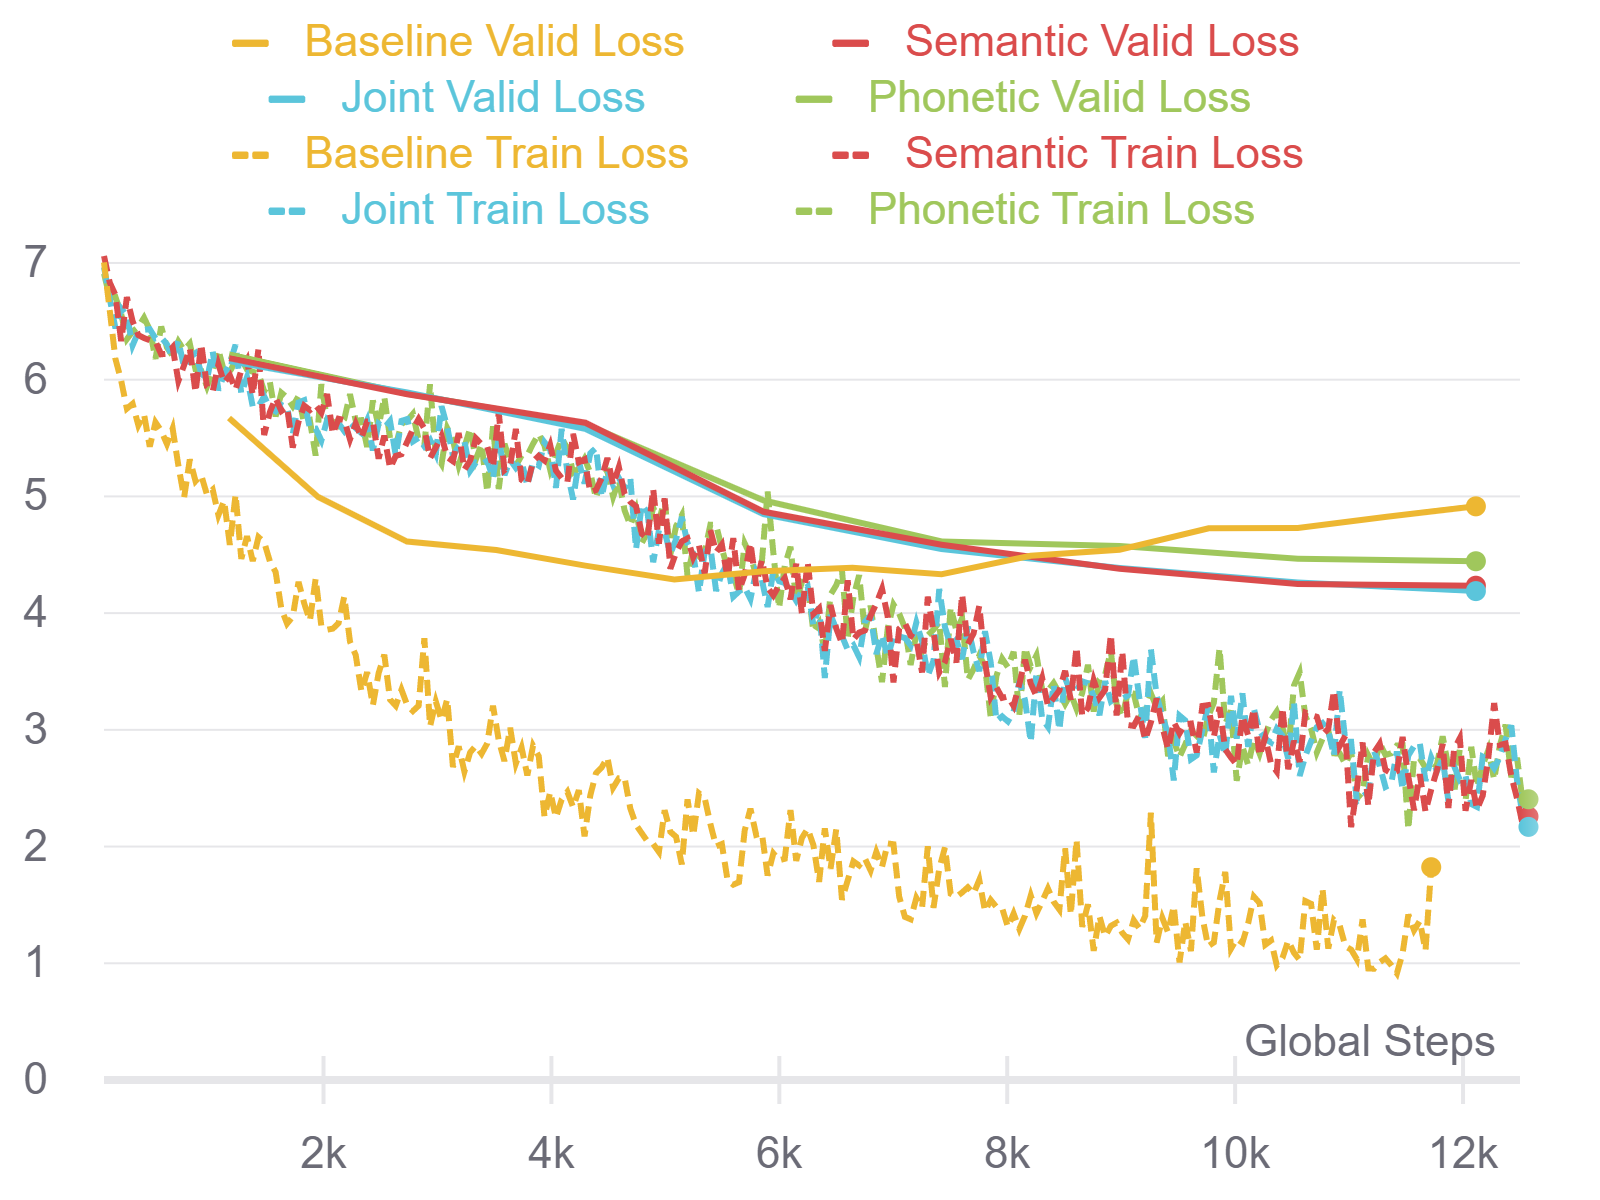
\includegraphics[width=\textwidth]{../images/rnn_jj.png}
        \caption{Results using Jieba \& Janome}
        \label{fig:seq2seq_loss_jj}
    \end{subfigure}
    \caption{Train and Validation Loss of Attention-based Bi-GRU Model}
	\label{fig:seq2seq_loss}
\end{figure}

Table~\ref{tab:seq2seq_bleu_score} shows the BLEU scores for all combinations on the attention-based Bi-GRU model. Using \texttt{SentencePiece} as a tokenizer scores about 4 to 5 lower than the average score of \texttt{Jieba} + \texttt{Janome}. This is reasonable because SentencePiece is a data-driven tokenizer, and the lack of data in the small corpus has largely hampered its ability to train embedding and NMT systems. The use of joint embedding successfully outperforms baseline and the other two embeddings based on both tokenization methods. Furthermore, it improves performance over baseline by about 2 BLEU points when using the \texttt{Jieba} and \texttt{Janome} tokenizers

\begin{table}[t]
    \centering
    \begin{tabularx}{\textwidth}{bbbbb}\toprule
        Tokenization & Baseline & Semantic & Phonetic & Joint \\\midrule
        SentencePiece & 21.63 & 21.66 & 21.32 & \textbf{22.33} \\
        Jieba + Janome & 25.16 & 26.71 & 26.18 & \textbf{27.05} \\\bottomrule
    \end{tabularx}
    \caption{BLEU Scores of Attention-based Bi-GRU Model}
    \label{tab:seq2seq_bleu_score}
\end{table}

\vspace{0.5cm}
\begin{figure}[t]
    \centering
    \begin{subfigure}[b]{0.495\textwidth}
        \centering
        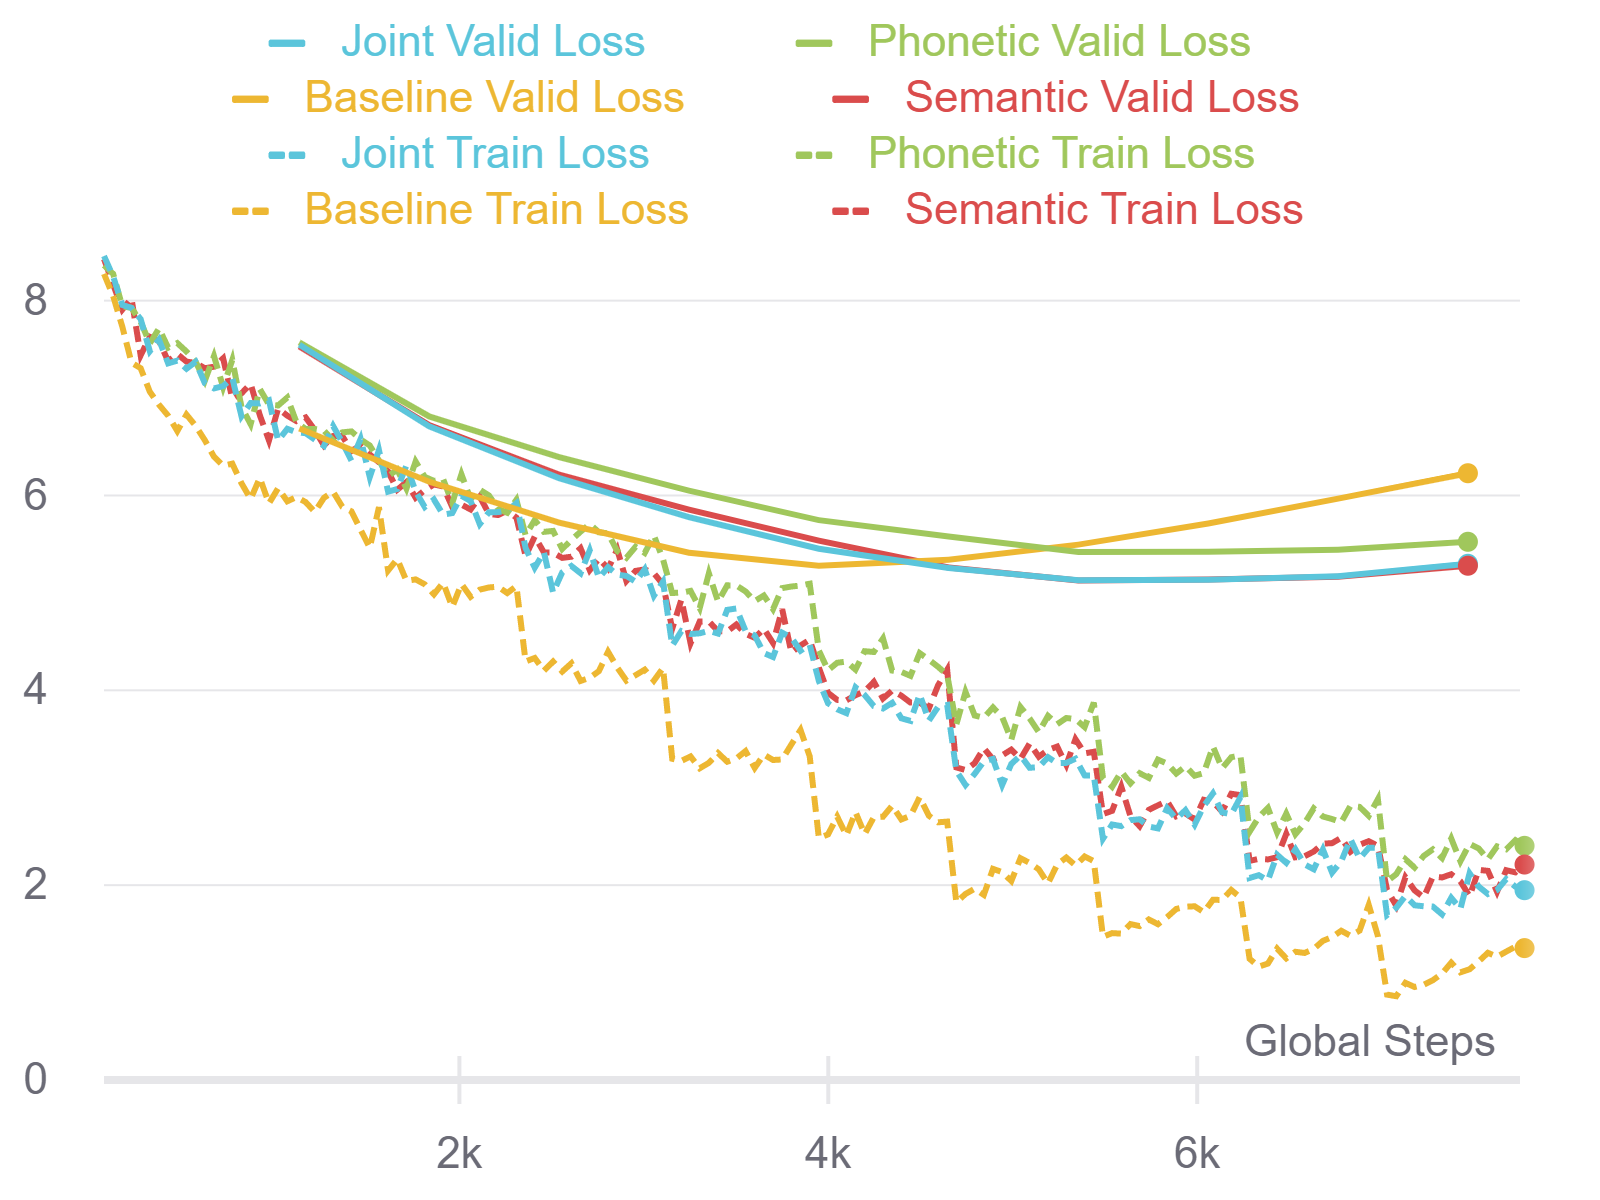
\includegraphics[width=\textwidth]{../images/transformer_sp.png}
        \caption{The results using SentencePiece}
        \label{fig:transformer_loss_sp}
    \end{subfigure}
    \hfill
    \begin{subfigure}[b]{0.495\textwidth}
        \centering
        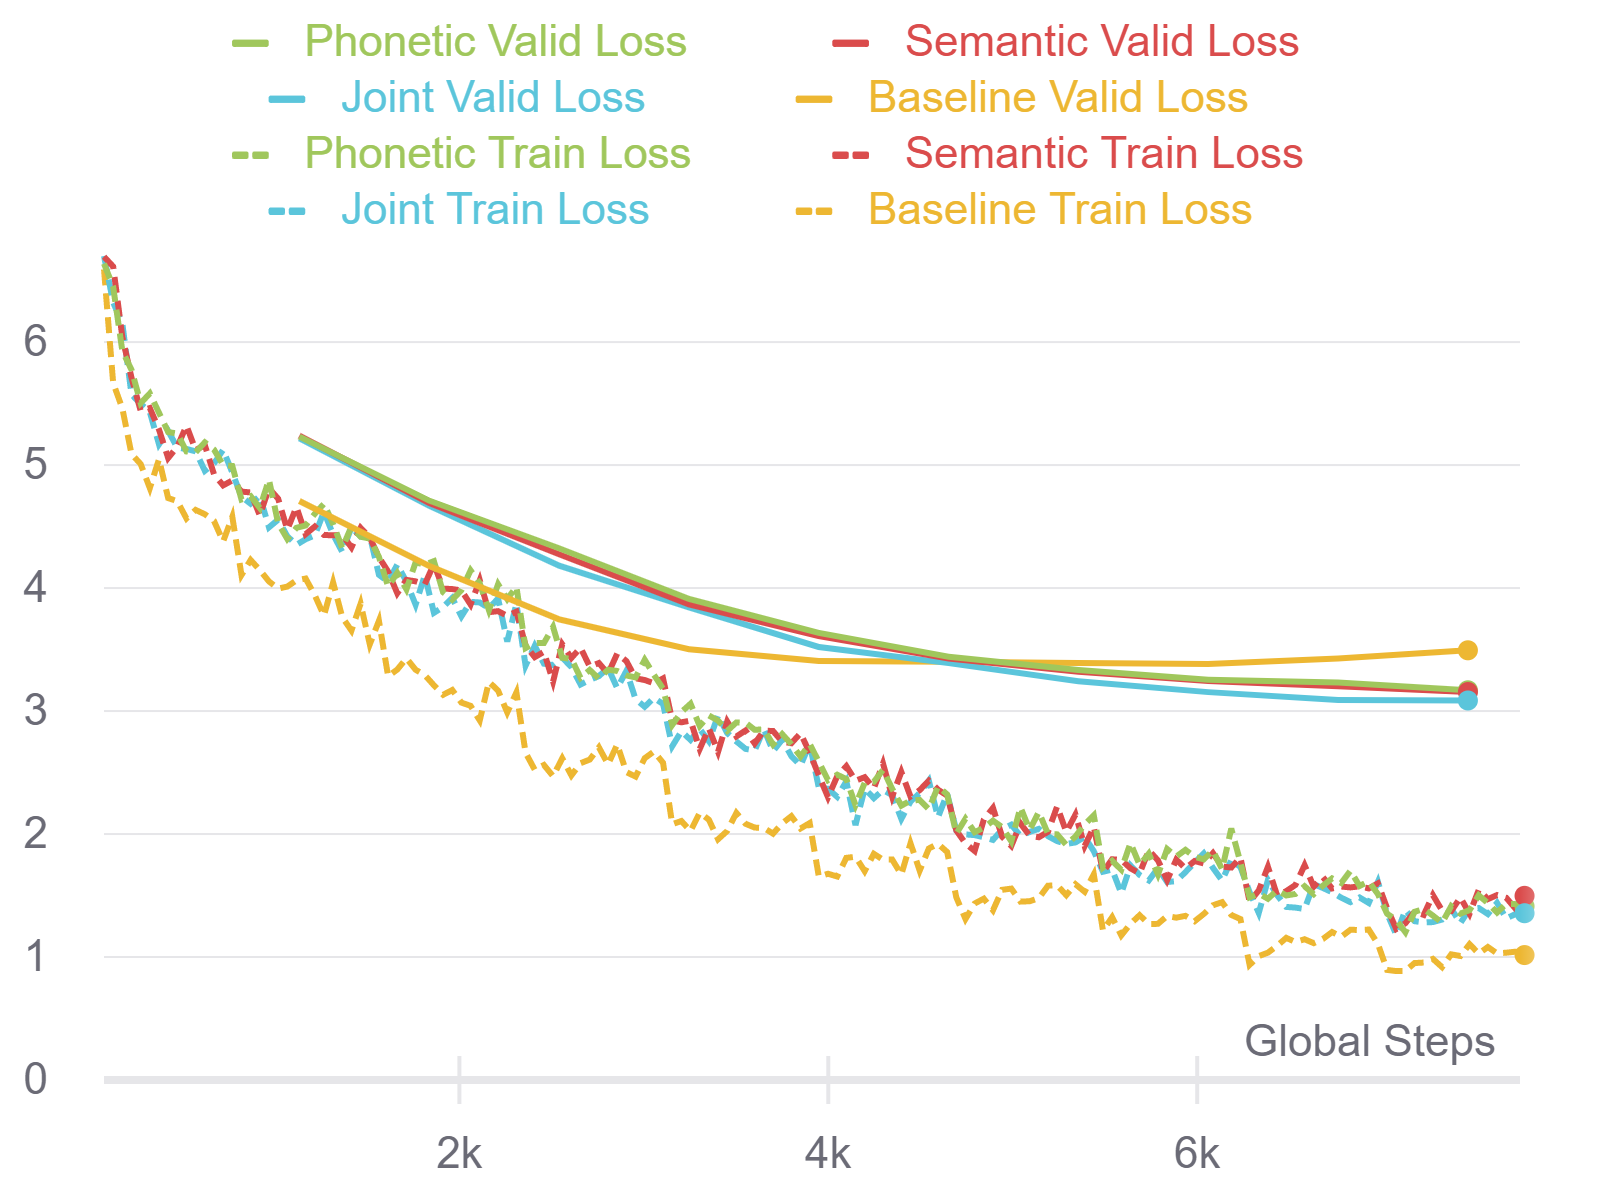
\includegraphics[width=\textwidth]{../images/transformer_jj.png}
        \caption{The results using Jieba \& Janome}
        \label{fig:transformer_loss_jj}
    \end{subfigure}
    \caption{Train and Validation Loss of Transformer}
	\label{fig:transformer_loss}
\end{figure}

\subsection{Transformer}

Figure~\ref{fig:transformer_loss} shows the losses of using the two tokenization methods on the Transformer. The addition of embeddings can resist overfitting in the Transformer as well as in the attention-based Bi-GRU Model. The semantic and joint embedding perform similarly when using \texttt{SentencePiece} as the tokenization method, but both are better than the embedding that only applies phonetic information (Figure~\ref{fig:transformer_loss_sp}). On the other hand, the joint embedding is a bit better than semantic and phonetic embedding with \texttt{Jieba} and \texttt{Janome} (Figure~\ref{fig:transformer_loss_jj}).

Table~\ref{tab:transformer_bleu_score} shows the BLEU scores for all combinations on the Transformer. The joint embedding obtains the highest scores with either \texttt{SentencePiece} or \texttt{Jieba} + \texttt{Janome} as the tokenization method. In the case of using \texttt{Jieba} and \texttt{Janome}, the joint embedding improves performance by 1 and 3 BLEU points respectively over the semantic embedding and baseline system.

\vspace{0.5cm}
\begin{table}[h]
    \centering
    \begin{tabularx}{\textwidth}{bbbbb}\toprule
        Tokenization & Baseline & Semantic & Phonetic & Joint \\\midrule
        SentencePiece & 24.32 & 25.72 & 23.48 & \textbf{26.44} \\
        Jieba + Janome & 29.31 & 31.23 & 30.90 & \textbf{32.48} \\\bottomrule
    \end{tabularx}
    \caption{BLEU Scores of Transformer}
    \label{tab:transformer_bleu_score}
\end{table}

\subsection{Best Model}

We decided to use \texttt{Jieba} + \texttt{Janome} as the base tokenization method to train and re-evaluate the four scenarios using the complete and filtered dataset with 462,582 sentence pairs. The results are shown in Table~\ref{tab:transformer_filtered_bleu_score}. The use of joint embedding still achieves the best BLEU score, which is 0.35 higher than the baseline system.

\vspace{0.5cm}
\begin{table}[h]
    \centering
    \begin{tabularx}{\textwidth}{bbbbb}\toprule
        Tokenization & Baseline & Semantic & Phonetic & Joint \\\midrule
        Jieba + Janome & 52.78 & 52.83 & 53.04 & \textbf{53.13} \\\bottomrule
    \end{tabularx}
    \caption{BLEU Scores of Transformer with Complete, Filtered Dataset}
    \label{tab:transformer_filtered_bleu_score}
\end{table}

We also used the baseline system of Workshop on Asian Translation 2020 (WAT) \cite{nakazawa2020overview} as a benchmark for evaluation, although we did not apply through its official submission system. For the ASPEC-JC task, WAT 2020 designed the baseline system using \texttt{OpenNMT} \footnote{https://github.com/OpenNMT/OpenNMT}, BPE, and attention mechanisms. The BLEU score and three different tokenization methods are used for evaluating Chinese to Japanese translation. As shown in Table~\ref{tab:wat_2020}, our best model (53.13) outperforms the baseline system of WAT 2020 by about 6 BLEU points with the enhancement of tokenization, embedding, corpus filtering, etc.

\vspace{0.5cm}
\begin{table}[h]
    \centering
    \begin{tabularx}{\textwidth}{bbbb}\toprule
         & Juman 7.0 & KyTea 0.4.6 & Mecab 0.996 \\\midrule
        Baseline & 46.87 & 47.30 & 47.00 \\
    \end{tabularx}
    \caption{BLEU Scores for the WAT2020 Baseline System}
    \label{tab:wat_2020}
\end{table}




